\section{Kiến trúc tổng thể hệ thống}
Hệ thống học tập trực tuyến thông minh được thiết kế theo mô hình Client – Server, với các thành phần chính bao gồm:

\subsection{Frontend (Client-side):}
Được xây dựng bằng Vue 3, giao diện người dùng cung cấp các tính năng như đăng nhập, học bài, làm bài tập, theo dõi tiến độ học tập, tương tác với gia sư AI, gửi phản hồi, \dots

Frontend giao tiếp với backend thông qua các API RESTful.

\subsection{Backend (Server-side):}
Đảm nhiệm xử lý logic nghiệp vụ, quản lý dữ liệu người dùng, khóa học, bài học, bài tập, tiến độ học, phản hồi, \dots Đồng thời xử lý yêu cầu từ AI (qua LLM API).
Backend được xây dựng bằng FastAPI. 
\subsection{Cơ sở dữ liệu (Database):}
Sử dụng hệ quản trị cơ sở dữ liệu PostgreSQL để lưu trữ thông tin người dùng, khóa học, bài học, kết quả học tập, bài tập, phản hồi, \dots
Thiết kế cơ sở dữ liệu đảm bảo tính mở rộng, hỗ trợ việc theo dõi tiến độ và sinh báo cáo.

\subsection{AI Module (LLM – Large Language Model):}
Các tác vụ như gợi ý lộ trình học, sinh bài tập, chấm điểm và hỗ trợ giải thích được thực hiện nhờ tích hợp LLM API (OpenAI, Gemini)
Backend sẽ định nghĩa prompt phù hợp và gửi yêu cầu tới LLM để lấy kết quả.

\subsection{Hệ thống lưu trữ tài liệu:}
Các tài liệu PDF, slide bài giảng được lưu ở AWS S3 thư mục local server.

\section{Sơ đồ cơ sở dữ liệu}
\begin{figure}[H]
    \centering
    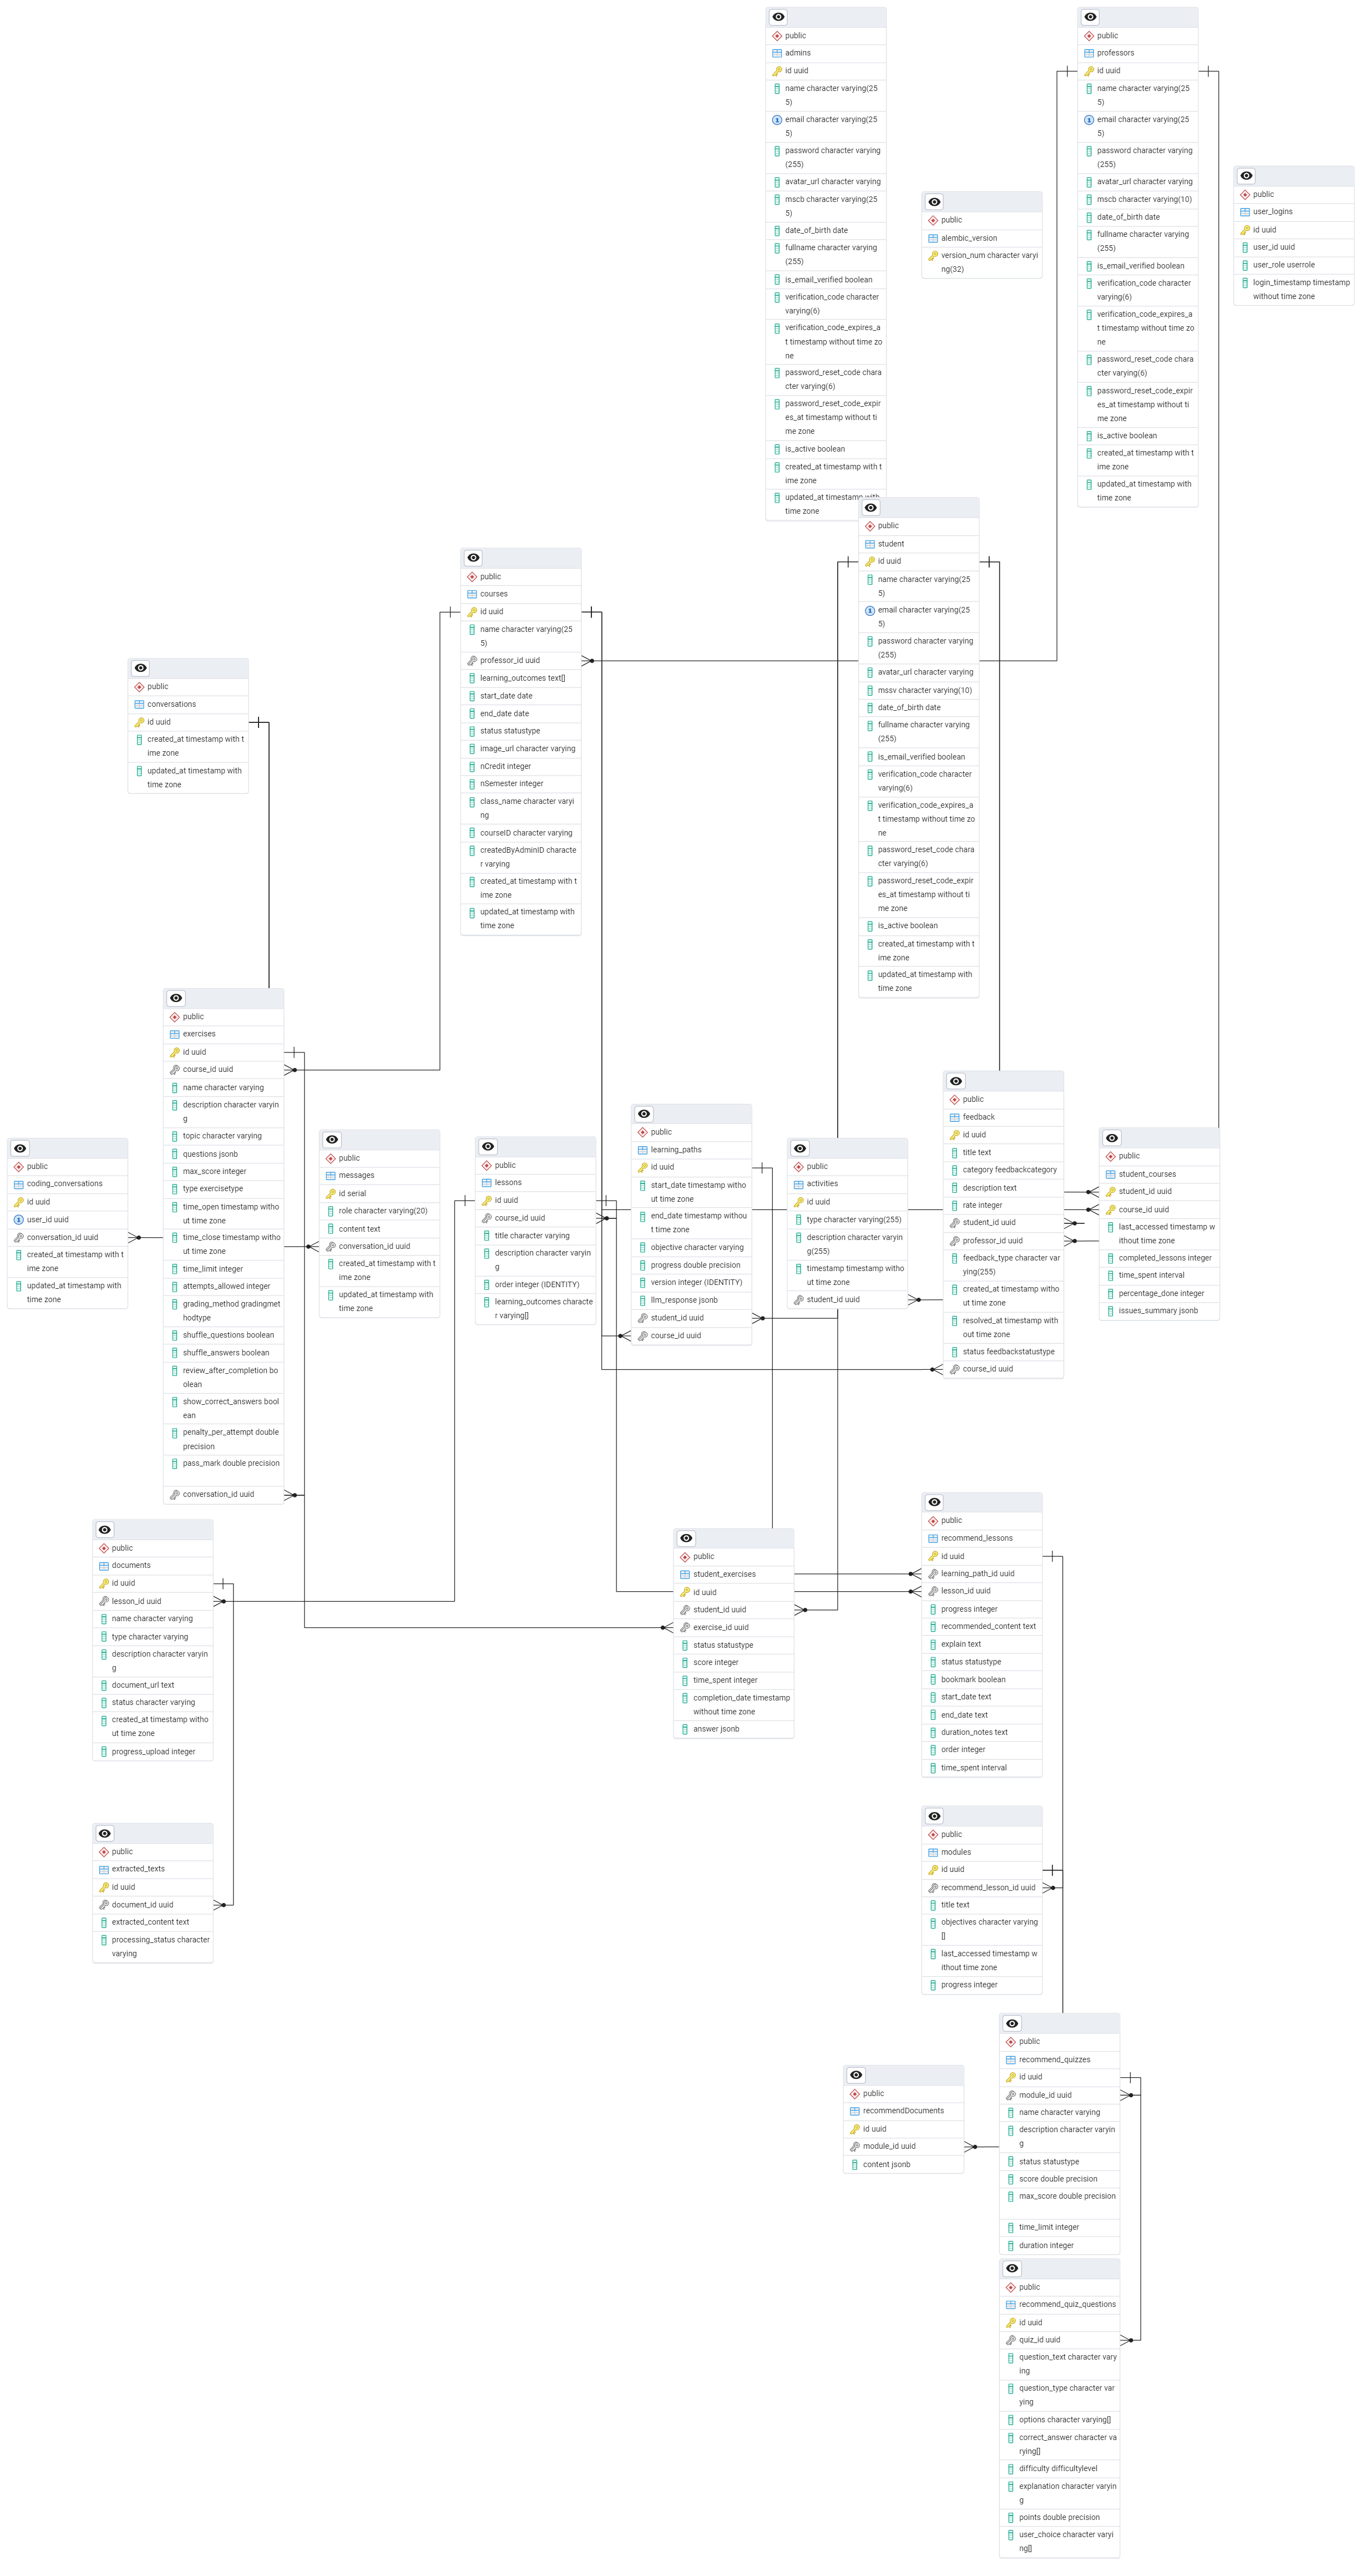
\includegraphics[width=0.6\linewidth]{images/ERD.png}
    \caption{Sơ đồ ERD của hệ thống}
    \label{fig:enter-label}
\end{figure}

\subsection{Tổng quan cấu trúc cơ sở dữ liệu}
Hệ thống được xây dựng trên nhiều bảng chính, chia thành các nhóm chức năng như sau:

\subsubsection{Nhóm người dùng (User Management)}
\begin{itemize}
    \item \textbf{professors}, \textbf{student}, \textbf{admins}: chứa thông tin cơ bản của người dùng theo 3 role như username, email, password,...
    \item \textbf{user\_login}\: bảng mở rộng lưu thông tin đăng nhập người dùng.
\end{itemize}

\subsubsection{Nhóm khóa học và tài liệu (Course Management)}
\begin{itemize}
    \item \textbf{courses}, \textbf{student\_courses}, \textbf{extracted\_text}: quản lý thông tin khóa học, tham gia khóa học và tài liệu học tập liên quan do giảng viên đăng tải.
    \item \textbf{lessons}, \textbf{documents}, \textbf{modules}: quản lý bài học và các nội dung bài học liên quan.
    \item \textbf{learning\_paths}, \textbf{recommend\_lessons}, \textbf{recommend\_documents}: quản lý các bài kiểm tra, bài tập và câu hỏi liên quan đến khóa học.
\end{itemize}

\subsubsection{Nhóm câu hỏi và bài kiểm tra (Assessment)}
\begin{itemize}
    \item \textbf{recommend\_quizzes}, \textbf{exercises}: chứa thông tin về các câu hỏi, loại câu hỏi, câu trả lời và kết quả bài kiểm tra của sinh viên trong các bài quiz được sinh ra theo từng bài học đề xuất.
\end{itemize}

\subsubsection{Nhóm tương tác và phản hồi (Interaction)}
\begin{itemize}
    \item  \textbf{feedbacks}, \textbf{activities}: quản lý tương tác giữa sinh viên và giảng viên, người dùng và hệ thống, và các hoạt động của người dùng.
\end{itemize}

\subsubsection{Nhóm bài tập Code Exercises}
\begin{itemize}
    \item \textbf{conversations}, \textbf{messages}, \textbf{coding\_conversations}: ghi nhận nhật ký hoạt động, cài đặt hệ thống và quản lý phiên làm việc.
\end{itemize}

\subsection{Mối quan hệ giữa các bảng}
Các bảng trong hệ thống có mối quan hệ nhiều-nhiều và một-nhiều, với các khóa ngoại được thể hiện rõ trong sơ đồ:
\begin{itemize}
    \item Một người dùng có thể tham gia nhiều khóa học thông qua bảng \texttt{student\_courses}.
    \item Một khóa học có thể có nhiều bài học, bài kiểm tra và tài liệu.
    \item Bài kiểm tra có thể bao gồm nhiều câu hỏi và mỗi câu hỏi có nhiều đáp án.
    \item Người dùng có thể đưa ra phản hồi và nhận thông báo từ hệ thống.
    \item Một sinh viên đối với một khóa học có thể có nhiều lộ trình học khác nhau. 
    \item Một lộ trình học có thể có nhiều bài học và tài liệu khác nhau.
    \item Một bài học có thể có nhiều module nhỏ và nội dung khác nhau.
    \item Một module có thể có nhiều bài quiz hoặc code exercises khác nhau (do sinh viên tùy chọn sinh ra)
\end{itemize}

\subsection{Kết luận}
Sơ đồ ERD này cung cấp một cái nhìn toàn diện về kiến trúc cơ sở dữ liệu của hệ thống. Cấu trúc được tổ chức hợp lý, cho phép dễ dàng mở rộng và tích hợp thêm các chức năng mới như AI hỗ trợ học tập, phân tích dữ liệu học viên, và hơn thế nữa.
